\documentclass{beamer}
\usetheme{Dresden}
\usecolortheme{dove}
%% Checking if saving file is working more
%\usepackage{graphicx} %For jpg figure inclusion
%\usepackage{times} %For typeface
%\usepackage{epsfig}
\usepackage{color} %For Comments
\usepackage{beamerthemeshadow} %Paul and Lemmon put this in, take out if you want
\usepackage{tikz}
%\usepackage[all]{xy}
%\usepackage{float}
%\usepackage{subfigure} 
%\usepackage{hyperref}
%\usepackage{url}
%\usepackage{parskip}
%\usepackage{multirow}
\usepackage{fancyvrb}
\fvset{fontsize=\normalsize}
\RecustomVerbatimEnvironment{verbatim}{Verbatim}{} 	

\definecolor{ForestGreen}{RGB}{34,139,34}
\definecolor{BestBlue}{RGB}{80,200,200}
% Uncomment this if you want to show work-in-progress comments
\newcommand{\comment}[1]{{\bf \tt  {#1}}}
% Uncomment this if you don't want to show comments
%\newcommand{\comment}[1]{}
\newcommand{\emcomment}[1]{\textcolor{ForestGreen}{\comment{Elena: {#1}}}}
\newcommand{\todo}[1]{\textcolor{blue}{\comment{To Do: {#1}}}}
\newcommand{\thcomment}[1]{\textcolor{BestBlue}{\comment{Thomas: {#1}}}}
\newcommand{\rmcomment}[1]{\textcolor{magenta}{\comment{Ryan: {#1}}}}
%%%%%%%%%%%%%%%%%%%%%%%%%%%%%%%%%%%%%%%%%%

\begin{document}
\author{Elena Machkasova, Thomas Hagen, Ryan McArthur}
\title{Super-fun with First-class Shapes in Quil}
\date{Clojure/conj: November 16, 2015}
\institute{University of Minnesota, Morris}


\begin{frame}
\frametitle {Super-fun with First-class Shapes in Quil}
\maketitle
\end{frame}
%frame

\begin{frame}
\frametitle{Table of contents}
\tableofcontents  
\end{frame}

\section{Overview}

\subsection{Who we are and why we are here}

\begin{frame}
\frametitle{Where are we from?}
\begin{figure}[h]

\includegraphics[width=7cm]{PresentationImages/umm-winter.jpg}
\end{figure}
UMM is a small liberal arts campus of UMN located 3 hours driving from Minneapolis/St.Paul. 
\end{frame}

\begin{frame}
\frametitle{What are we working on?}
Specific goal: developing Clojure-based introductory CS course ({\it \href{http://cda.morris.umn.edu/~elenam/\#clojure}{ClojurEd project}}). 

General goal: making Clojure more accessible to beginners and those with no Java background. 

What does this include? 
\begin{enumerate}
\item Beginner-friendly error messages. 
\item Libraries and tools that allow beginners to explore functional approaches, recursion, and abstraction.
\item Integration into a beginner-friendly IDE. 
\end{enumerate}
\end{frame}

\begin{frame}
\frametitle{What are we working on?}
Developing Clojure-based introductory CS course ({\it \href{http://cda.morris.umn.edu/~elenam/\#clojure}{ClojurEd project}}). 

General goal: making Clojure more accessible to beginners and those with no Java background. 

What does this include? 
\begin{enumerate}
\item Beginner-friendly error messages. 
\item {\bf Libraries and tools that allow beginners to explore functional approaches, recursion, and abstraction: graphical library.}
\item Integration into a beginner-friendly IDE. 
\end{enumerate}
Summer project 2015. 
\end{frame}

\subsection{Wish-list for beginner-friendly graphical library}

\begin{frame}
\frametitle{Beginner-friendly graphical library}
Inspiration: Racket ``universe'' package \href{http://racket-lang.org/}{http://racket-lang.org/}
\begin{itemize}
\item Separation of Model, View, Control (MVC) 
\item Functional implementation of MVC: world state, functions: 

\noindent
old world state $\rightarrow$ new world state \\
world state $\rightarrow$ image 
\item  First-class shapes (circles, rectangles, user-added jpegs, etc) not attached to any position
\item Functions to combine simpler shapes into complex shapes: {\tt above, beside, overlay, scale...}
\end{itemize}
\end{frame}

\begin{frame}[fragile]
\frametitle{Beginner-friendly graphical library: MVC}
\begin{verbatim}
(define (main duration)
  (big-bang '() ; starts with an empty list of positions.
   [to-draw display-dots] ;draw dots on canvas
   [on-tick do-nothing 1 duration] ;dots don't move w/time
   [on-mouse add-or-remove-dot])) ;click handling
\end{verbatim}
\begin{figure}[h]
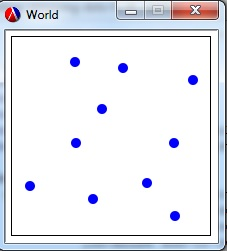
\includegraphics[width=4cm]{PresentationImages/dots.jpg}
\end{figure}
\end{frame}

\begin{frame}[fragile]
\frametitle{Beginner-friendly graphical library: first-class shapes}
\begin{verbatim}
(define dot (circle 10 "solid" "blue"))

;; display-dots: list of positions  -> image
(define (display-dots lop)     
  (cond [(empty? lop) blank-scene]
        [else (place-image dot
                           (posn-x (first lop))
                           (posn-y (first lop))
                           (display-dots (rest lop)))]))

;; add-or-remove-dot: list of positions, 
;; coordinates of click -> list of positions
.........
\end{verbatim}

\end{frame}

\section{Clojure first-class shapes}

\subsection{Functional MVC in Quil: fun-mode}


\begin{frame}
\frametitle{World States in Quil}
	\begin{itemize}
		\item  Using Nikita Beloglazov's  Quil fun-mode (functional MVC)
		\item State as a HashMap
	\end{itemize}
	\begin{figure}
		\includegraphics[width=8cm]{PresentationImages/setupCode.pdf}
	\end{figure}
	\begin{itemize}
		\item fun-mode + first class shapes = super-fun!
	\end{itemize}
\end{frame}

\begin{frame}
\frametitle{World States in Quil}
\begin{itemize}
		\item Elements of the state modified through functions
	\end{itemize}
	\begin{figure}
		\includegraphics[width=8cm]{PresentationImages/updateCode.pdf}
	\end{figure}
\end{frame}


\subsection{Ideas and examples}


\begin{frame}
\frametitle{Shapes as First Class Objects}
	\begin{itemize}
		\item Racket-style implementation of shapes
		\item Shapes are treated as objects, modified through functions
		\item Shapes hold their specifications for drawing
		\item Easy to redraw wherever needed
		\item Easier to understand conceptually for beginners
	\end{itemize}
\end{frame}

\begin{frame}
\frametitle{Creating a Collage}
	\begin{itemize}
		\item Functional Quil uses paintbrush approach
	\end{itemize}
	\begin{figure}
	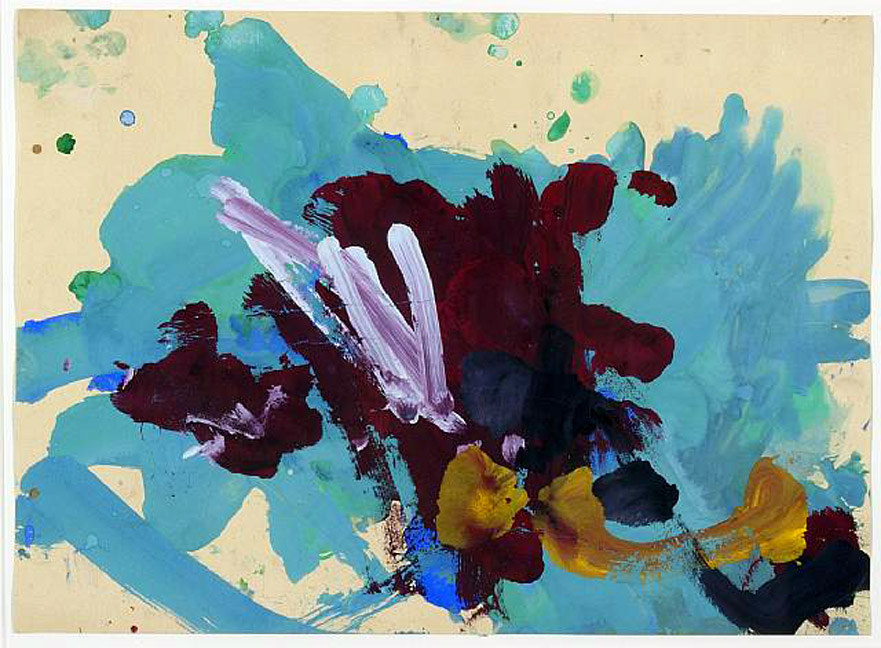
\includegraphics[width=3.5cm]{PresentationImages/painting.jpg}
	\end{figure}
	\begin{itemize}
		\item Our firstclass-shapes use collage approach
	\end{itemize}
	\begin{figure}
	\hspace{-1cm}
	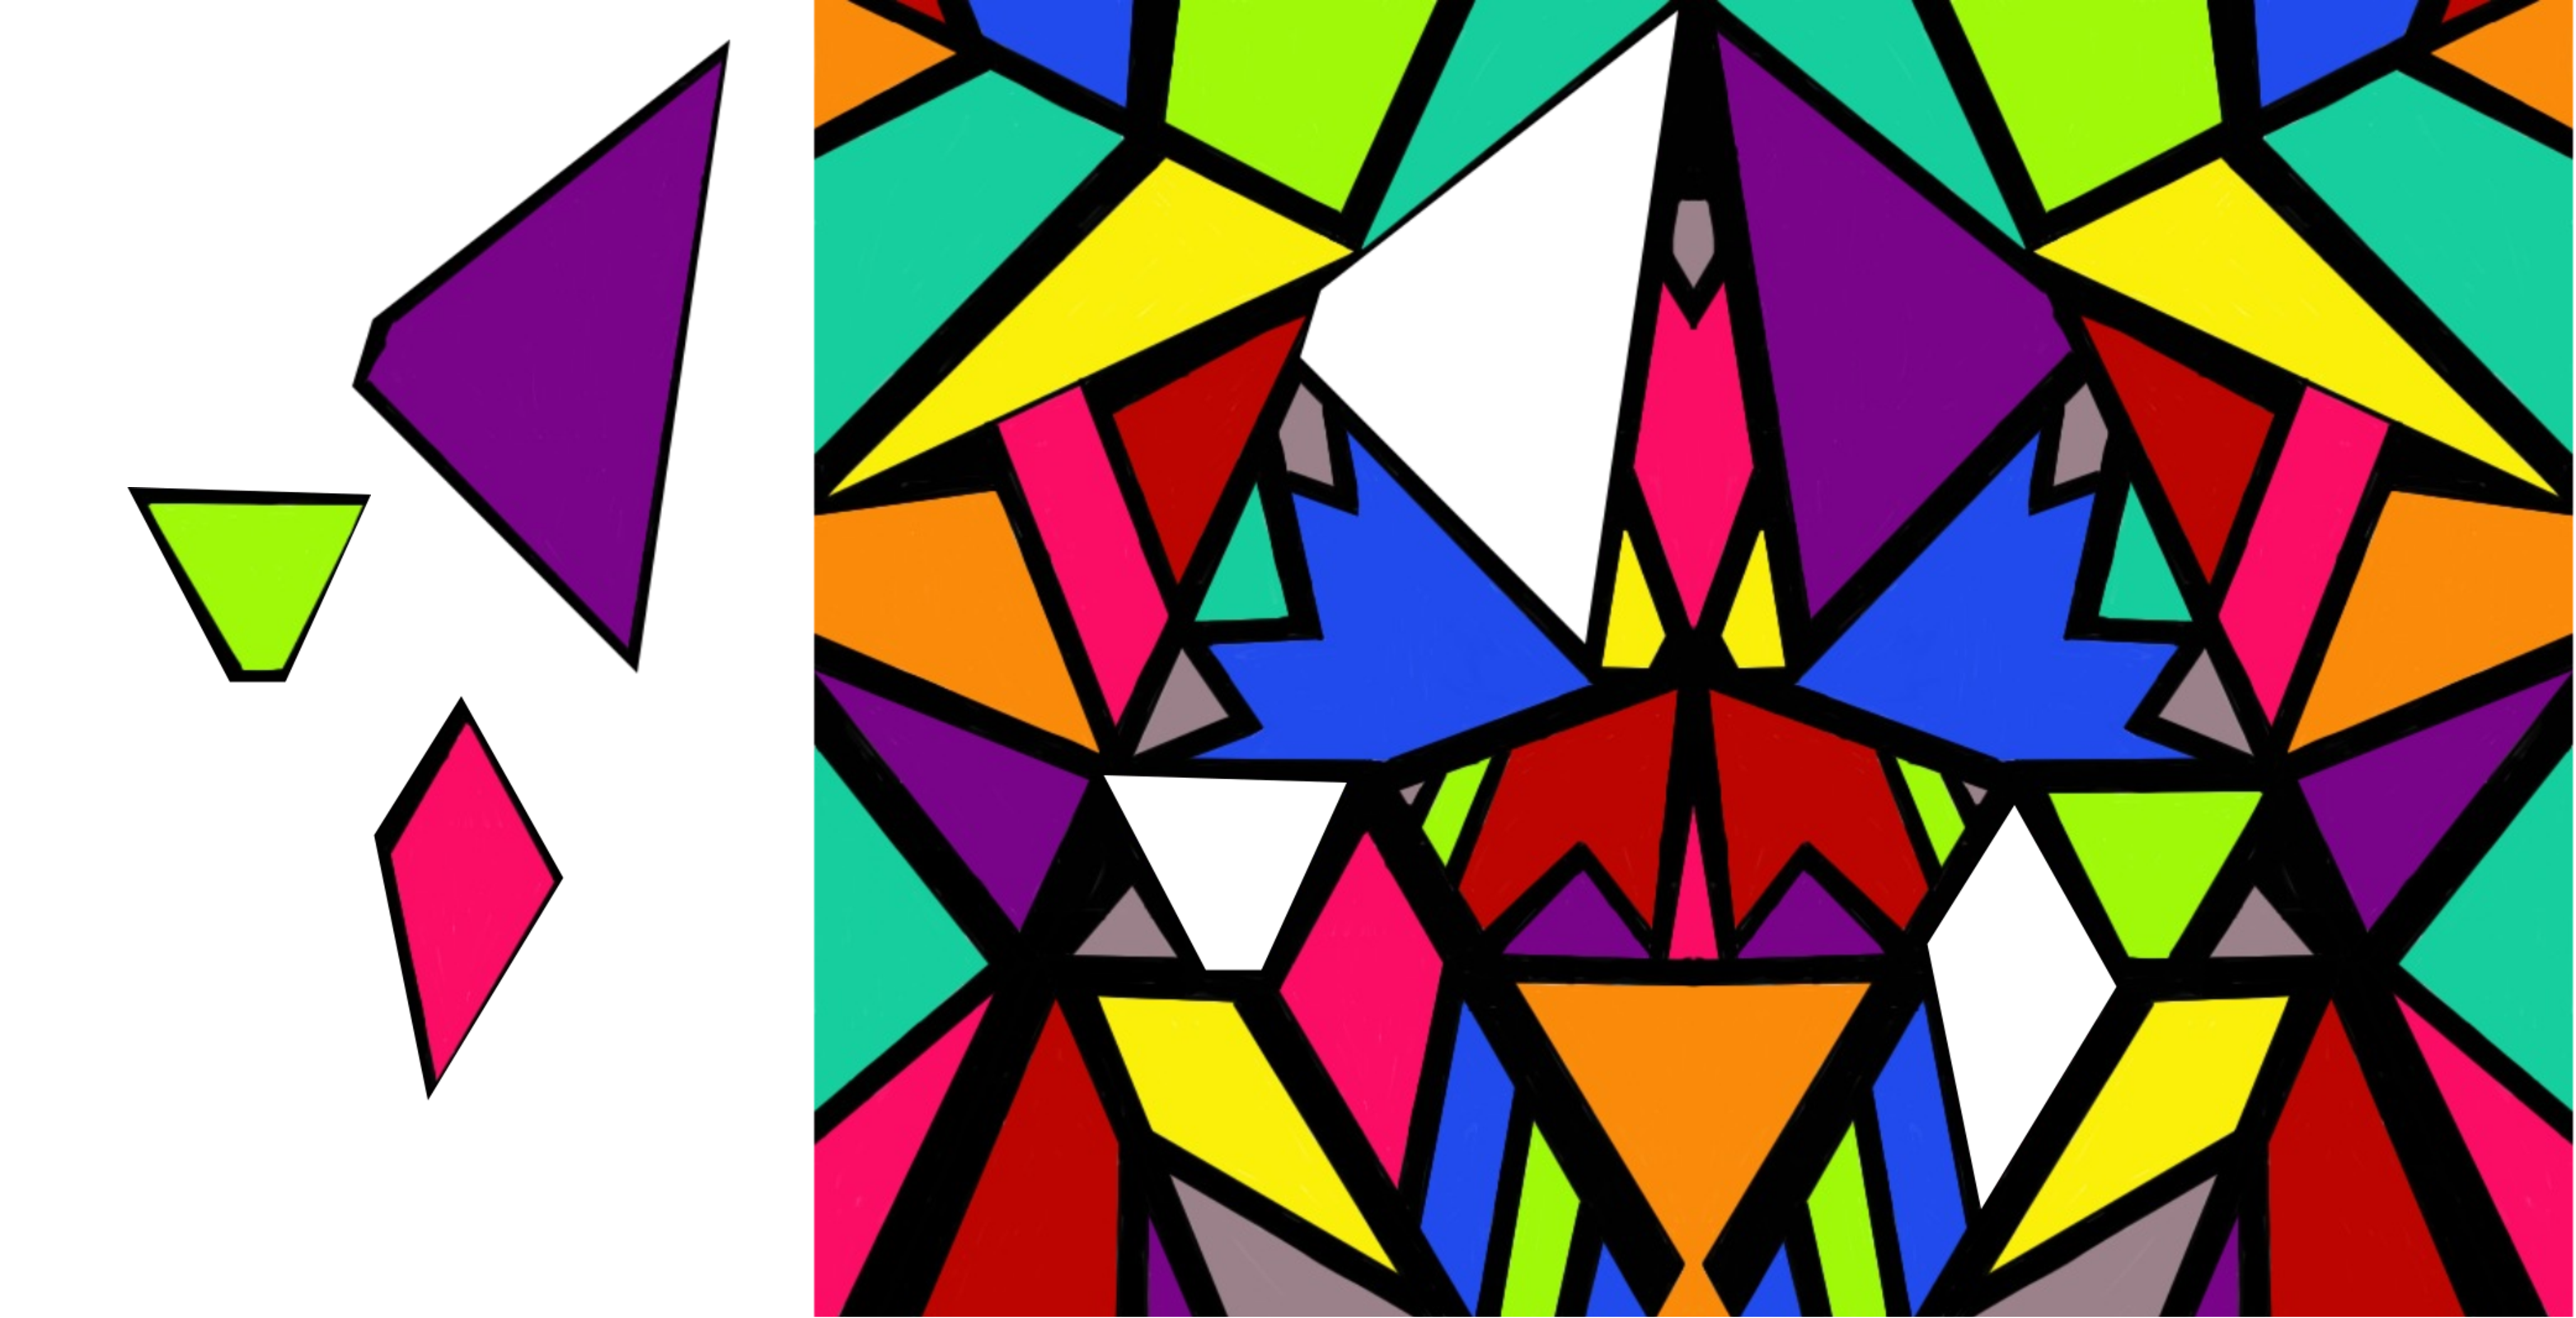
\includegraphics[width=4.5cm]{PresentationImages/collage2.pdf}
	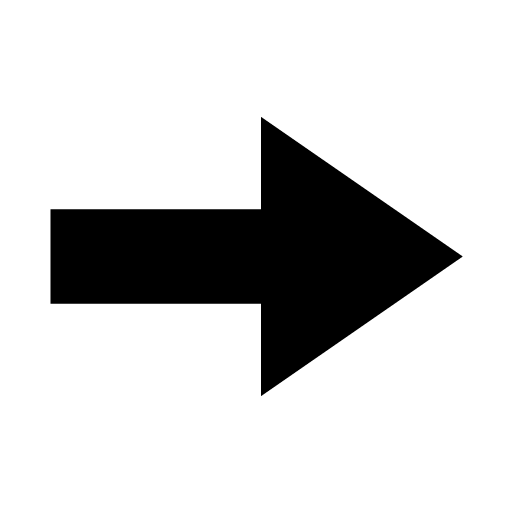
\includegraphics[width=2cm]{PresentationImages/blackArrow.png}
	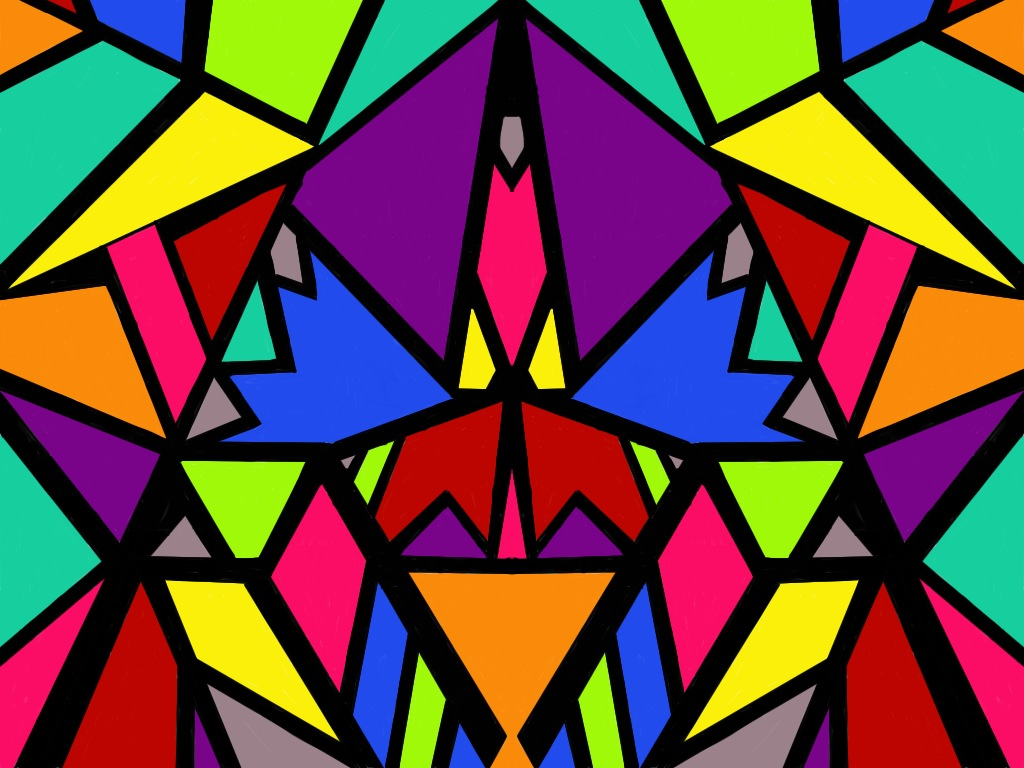
\includegraphics[width=3.1cm]{PresentationImages/collage.jpg}
	\end{figure}
\end{frame}

\begin{frame}
\frametitle{Simple Shapes}
	\begin{itemize}
		\item Quil shapes live in the draw function 
		\item Quil shapes do not exist until they are drawn. 
		\item The function to make a rectangle only draws the shape.
	\end{itemize}
	\begin{figure}
		\includegraphics[width=6cm]{PresentationImages/quilGreenRect.pdf}
		\hspace{1cm}
		\includegraphics[width=1.2cm]{PresentationImages/ourGreenRect.pdf}
	\end{figure}
\end{frame}

\begin{frame}
\frametitle{Our Shapes}
	\begin{itemize}
		\item Our shapes are defined once in setup and reused when needed
		\item Our shapes are drawn through the ds (draw-shape) function 
	\end{itemize}
	\begin{figure}
		\includegraphics[width=6cm]{PresentationImages/ourGreenRectCode.pdf}
		\hspace{1cm}
		\includegraphics[width=1.2cm]{PresentationImages/ourGreenRect.pdf}
	\end{figure}
\end{frame}

\begin{frame}
\frametitle{Complex Shapes}
	\begin{itemize}
		\item Complex shapes are a collection of simple shapes
		\item Each simple shape holds their individual offsets
		\item Methods are used to create complex shapes from simple ones
	\end{itemize}
	\begin{figure}
	\includegraphics[width=5cm]{PresentationImages/greenCircleRectangleCode.pdf}
	\hspace{1cm}
	\includegraphics[width=4cm]{PresentationImages/greenCircleRectangle.pdf}
	\end{figure}
\end{frame}

\begin{frame}
\frametitle{Above and Beside}
	\begin{itemize}
		\item Complex shapes are constructed through calling above or beside
		\item Reduce can be used for similar effect
	\end{itemize}

	\begin{figure}
	\hspace{-4.3cm}
	\vspace{0.8cm}
		\includegraphics[width=5.7cm]{PresentationImages/greenScaleRects.pdf}
	\end{figure}
	\begin{figure}
	\vspace{-4.8cm}
		\includegraphics[width=6.9cm]{PresentationImages/greenScaleRectsReduce.pdf}
		\hspace{1.6cm}
		\includegraphics[width=1.3cm]{PresentationImages/greenScaleTower.pdf}
	\end{figure}

\end{frame}

\begin{frame}
	\begin{itemize}
		\item And now for a successful live demo
	\end{itemize}
\end{frame}


\begin{frame}
\frametitle{Combining Complex Shapes}
	\begin{itemize}
		\item Combining complex shapes creates a new complex shape
		\begin{figure}
			\vspace{.5cm}
			\begin{figure}
				\hspace{3.7cm}
				\vspace{-.5cm}
				\includegraphics[width=6.2cm]{PresentationImages/complexStructure.pdf}
			\end{figure}
			\includegraphics[width=3.5cm]{PresentationImages/twoComplexCode.pdf}
			\hspace{0.3cm}
			\includegraphics[width=5.5cm]{PresentationImages/twoComplex.pdf}
		\end{figure}
	\end{itemize}
\end{frame}

\begin{frame}
\frametitle{Overlay}
	\begin{itemize}
		\item Complex shapes are also constructed through overlay
	\end{itemize}
	\begin{figure}
	\includegraphics[width=6cm]{PresentationImages/greenHoleCode.pdf}
	\hspace{1cm}
	\vspace{2cm}
	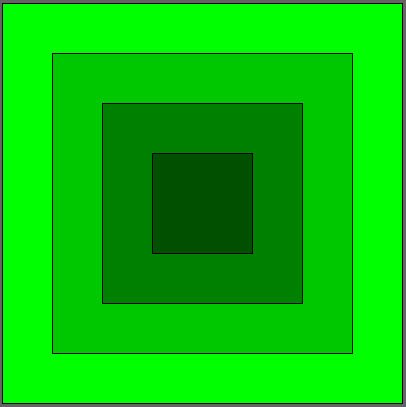
\includegraphics[width=3.5cm]{PresentationImages/greenHole.png}
	\end{figure}
\end{frame}

\begin{frame}
\frametitle{Align}
	\begin{itemize}
		\item An align version of overlay, above, and beside exist
	\end{itemize}
		\begin{figure}
		\includegraphics[width=5cm]{PresentationImages/greenLeanRightCode.pdf}
		\hspace{0.1cm}
		\includegraphics[width=5.5cm]{PresentationImages/greenAlignBottomRightCode.pdf}
	\end{figure}

	\begin{figure}
		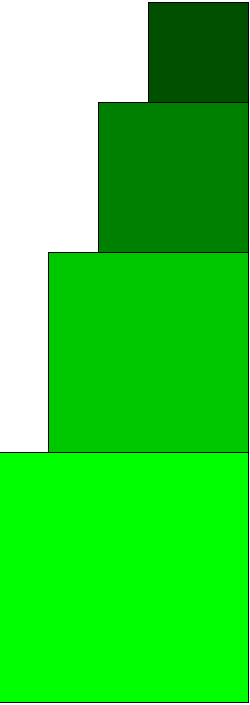
\includegraphics[width=1.0cm]{PresentationImages/greenLeanRight.png}
		\hspace{4cm} 	\vspace{0.3cm}
		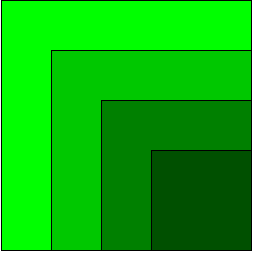
\includegraphics[width=2cm]{PresentationImages/greenAlignBottomRight.png}
	\end{figure}
\end{frame}

\begin{frame}[fragile]
\frametitle{Rotation and Scaling}
	\begin{itemize}
	\item You can modify the size and orientation of the shape
	\begin{columns}[t]
		\begin{column}{.45\textwidth}
			\begin{figure}[h]
				\hspace{0.25cm}
			\includegraphics[width=4cm]{PresentationImages/rotateRedCode.pdf}
			\end{figure}
		\end{column}
		\begin{column}{.3\textwidth}
			\begin{figure}[h]
			
\includegraphics[width=0.8cm]{PresentationImages/red-rectangle-rotate.png}
			\end{figure}		
		\end{column}
		\end{columns}
		
		\begin{columns}[t]
		\begin{column}{.45\textwidth}
			\begin{figure}[h]
			\hspace{0.25cm}
			\includegraphics[width=4.2cm]{PresentationImages/scaleRedCode.pdf}
			\end{figure}
		\end{column}
		\begin{column}{.3\textwidth}
			\begin{figure}[h]
			
\includegraphics[width=1.2cm]{PresentationImages/red-rectangle-scale.png}
			\end{figure}		
		\end{column}
		\end{columns}
		
		\begin{columns}[t]
		\begin{column}{.45\textwidth}
			\begin{figure}[h]
			\vspace{-0.5cm}
			\includegraphics[width=6.5cm]{PresentationImages/rotateAndScaleRedCode.pdf}
			\end{figure}
		\end{column}
		\begin{column}{.3\textwidth}
			\begin{figure}[h]
			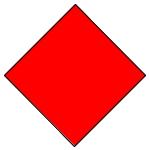
\includegraphics[width=1.7cm]{PresentationImages/red-rectangle-scale-rotate.png}
			\end{figure}		
		\end{column}
		\end{columns}
	\end{itemize}
\end{frame}

\begin{frame}
\frametitle{Images}
	\begin{itemize}
		\item images can be rotated and scaled similar to shapes
	\end{itemize}
	\begin{figure}
		\vspace{0.2cm}
		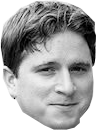
\includegraphics[width=1cm]{PresentationImages/kappa96x130.png}
		\hspace{0.4cm}
		\includegraphics[width=6cm]{PresentationImages/pictureOnBoxCode.pdf}
		\hspace{0.4cm}
		%\vspace{-3cm}
		\includegraphics[width=2cm]{PresentationImages/onBoxKappa.pdf}
	\end{figure}
\end{frame}

\begin{frame}
\frametitle{Code Comparison}
	\begin{itemize}
		\item Quil code vs our code 
	\end{itemize}
	\begin{figure}
	\hspace{-0.4cm}
	\includegraphics[width=3cm]{PresentationImages/theirRingsCode.pdf}
	\hspace{0.1cm}
	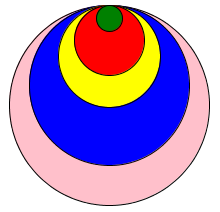
\includegraphics[width=2cm]{PresentationImages/rings.png}
	\hspace{0.1cm}
	\includegraphics[width=5.5cm]{PresentationImages/ourRingsCode.pdf}
	\end{figure}
\end{frame}


\subsection{Implementation}


\begin{frame}
\frametitle{Simple Shape Structure}
	\begin{itemize}
		\item As a data structure, simple shapes are hashes
		\item Shapes hold a variety of information within them
	\end{itemize}
	\begin{figure}
		\includegraphics[width=9cm]{PresentationImages/rectHashmap.pdf}
	\end{figure}
\end{frame}

\begin{frame}
\frametitle{Complex Shape Structure}
	\begin{itemize}
		\item Complex shapes are vectors of simple shapes
		\item Each shape knows its position from the center of the shape
		\item This is different from Racket's implementation.
		\item This allows for the ability to alter individual simple shapes.
	\end{itemize}
\end{frame}

\begin{frame}
	\begin{itemize}
		\item And now for another successful live demo
	\end{itemize}
\end{frame}

\begin{frame}
\frametitle{Draw-Shape Structure}
	\begin{itemize}
		\item Draw-shape calls the internal Quil draw function within the shape object
		\item Draw-shape also works on image objects
	\end{itemize}
	\begin{figure}
		\includegraphics[width=11cm]{PresentationImages/dsCode.pdf}
	\end{figure}
\end{frame}

\section{Future work}

\begin{frame}
	\frametitle{Future Work}
	\begin{itemize}
		\item Make it easy to get the color information from shapes (currently color is hard-wired in drawing function) 
		\item Add more functionality
		\begin{itemize}
			\item Add the ability to get the color of a simple shape
			\item Rotate complex shapes
			\item Pixel-detail Overlay and Overlay-Align
			\item Add support for text, textareas, etc.  
			\item More seamless integration with Quil fun-mode
		\end{itemize}
		\item Add examples to the git repo 
		\item Wish-list: Integrate overtone (music library)
	\end{itemize}
\end{frame}

\begin{frame}
	\frametitle{Where to find it}
	\begin{itemize}
	\item Clojars Page
	\href{https://clojars.org/org.clojars.quil-firstclass-shapes/firstclassshapes}{https://clojars.org/org.clojars.quil-firstclass-shapes/firstclassshapes}
	
	\href{https://clojars.org/org.clojars.quil-firstclass-shapes/firstclassshapes} {[org.clojars.quil-firstclass-shapes/firstclassshapes "0.0.1"]}
	
	\item Github Page
	\href{https://github.com/Clojure-Intro-Course/quil-firstclass-shapes}{https://github.com/Clojure-Intro-Course/quil-firstclass-shapes}
	\end{itemize}
	
\includegraphics[width=5cm]{PresentationImages/github.png}
	\hspace{1cm}
	
\includegraphics[width=4cm]{PresentationImages/clojars.png}
\end{frame}

\begin{frame}
	\frametitle{Similar Work}
Similar (completely independent) work: first-class shapes by Tom Hall, EuroClojure 2014, based on geomlab library. 

Used for educational purposes (just like ours).
%\begin{figure}
%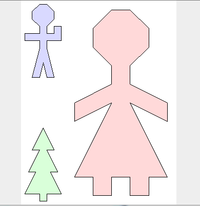
\includegraphics[width=4cm]{PresentationImages/geomlab.png}
%\end{figure}
\end{frame} 

\begin{frame}
\frametitle{Acknowledgments}
	{\large Thanks to:}
	\begin{figure}
		Morris-HHMI summer undergraduate research program at UMM 
\includegraphics[width=10cm]{PresentationImages/logoHHMI.jpg}
	\end{figure}
	\begin{figure}
		NSF North Star Stem Alliance/LSAMP grant 
		
\includegraphics[width=11cm]{PresentationImages/logoStem.jpg}
	\end{figure}	
	{\centering \qquad Clojure/conj organizers and sponsors!}
\end{frame}

\begin{frame}[fragile]
\frametitle{Questions?}

\begin{tikzpicture}[remember picture,overlay]
\node at (current page.center) {\includegraphics[width=3cm]{PresentationImages/qMarkgrey.png}};
\end{tikzpicture}
\begin{verbatim}[fontsize=\tiny]
(defn setup []
   (q/frame-rate 60)
   (q/color-mode :rgb)
   (def big-arc (create-arc 200 200 (- (/ q/PI -2) 0.9) (/ q/PI 2) 50))
   (def little-circle (create-ellipse 80 80 255))
   (def small-rect (create-rect 50 50 50))
   (def white-space (create-rect 50 25 255))
   (def big-rect (create-rect 50 60 50))
   (def q-mark (above (overlay-align :bottom :center
                                      big-rect
                                      (overlay 
                                      little-circle
                                               big-arc))
                       big-rect
                       white-space
                       small-rect))
    {})
  
  (defn update-state [state] {})


 (defn draw-state [state]
  (q/background 255)
  (q/no-stroke)
  (ds q-mark 500 500))
\end{verbatim}
	%\begin{figure}
		%
\includegraphics[width=1cm]{PresentationImages/qMarkBlack.png}
		%
\includegraphics[width=2cm]{PresentationImages/qMarkBlack2.png}
		%
\includegraphics[width=3cm]{PresentationImages/qMarkGrey.png}
		%
\includegraphics[width=4cm]{PresentationImages/qMarkGrey2.png}
	%\end{figure}
\end{frame}
\end{document}